\documentclass[tikz,dvipsnames]{standalone}
%\usepackage{tikz}
\usepackage{tikz-3dplot}
\usepackage{wasysym}

\begin{document}
\tdplotsetmaincoords{65}{130}
%
\pgfmathsetmacro{\rvec}{0.8}
\pgfmathsetmacro{\thetaJNvec}{40}
\pgfmathsetmacro{\thetaJLvec}{20}

\pgfmathsetmacro{\phivec}{20}
\pgfmathsetmacro{\phiNvec}{80}

\pgfmathsetmacro{\longascnode}{25}

\pgfmathsetmacro{\wfl}{\rvec}
\newcommand{\wfcolor}{gray}

\pgfmathsetmacro{\psil}{\wfl}
\pgfmathsetmacro{\psivec}{-30}

\pgfmathsetmacro{\orbitl}{0.5*\psil}

\pgfmathsetmacro{\discrad}{\rvec}

\newcommand*\lateraleye{%
\scalebox{0.15}{
\tikzset{every picture/.style={line width=0.75pt,-}} 
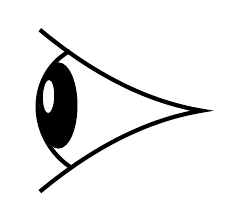
\begin{tikzpicture}[x=0.75pt,y=0.75pt,yscale=-1,xscale=1]
\draw  [-,line width=1.5]  (300,100.33) .. controls (326,122) and (352,135) .. (378,139.33) .. controls (352,143.67) and (326,156.67) .. (300,178.33) ;
\draw  [-,fill={rgb, 255:red, 0; green, 0; blue, 0 }  ,fill opacity=1 ] (308.94,116.33) .. controls (313.87,116.33) and (317.86,125.51) .. (317.85,136.83) .. controls (317.84,148.15) and (313.84,157.33) .. (308.91,157.33) .. controls (303.99,157.32) and (300,148.14) .. (300.01,136.82) .. controls (300.02,125.5) and (304.02,116.32) .. (308.94,116.33) -- cycle ;
\draw  [-,draw opacity=0][line width=1.5]  (314.84,166.6) .. controls (311.87,164.64) and (309.14,162.18) .. (306.76,159.24) .. controls (295.12,144.82) and (296.6,124.33) .. (310.07,113.45) .. controls (311.48,112.32) and (312.96,111.33) .. (314.5,110.49) -- (331.14,139.55) -- cycle ; \draw  [line width=1.5]  (314.84,166.6) .. controls (311.87,164.64) and (309.14,162.18) .. (306.76,159.24) .. controls (295.12,144.82) and (296.6,124.33) .. (310.07,113.45) .. controls (311.48,112.32) and (312.96,111.33) .. (314.5,110.49) ;
\draw  [-,fill={rgb, 255:red, 255; green, 255; blue, 255 }  ,fill opacity=1 ] (304.43,124.2) .. controls (306.09,124.25) and (307.32,128.01) .. (307.18,132.6) .. controls (307.05,137.19) and (305.59,140.88) .. (303.93,140.83) .. controls (302.27,140.78) and (301.03,137.02) .. (301.17,132.43) .. controls (301.31,127.83) and (302.76,124.15) .. (304.43,124.2) -- cycle ;
\end{tikzpicture}
}\,}

%
\begin{tikzpicture}[scale=5,tdplot_main_coords]
    \coordinate (O) at (0,0,0);
    \draw[thick,->,opacity=0.25] (0,0,0) -- (0,0,\rvec) node[anchor=south]{$\hat{J}$};

    \draw[thick,->, black,opacity=0.25] (O) -- ({\discrad*cos(90-\phiNvec)},{-\discrad*sin(90-\phiNvec)},0) node[anchor=north]{$\hat{x}_J$};
    \draw[thick,->, black,opacity=0.25] (O) -- ({\discrad*cos(\phiNvec)},{\discrad*sin(\phiNvec)},0) node[anchor=north]{$\hat{y}_J$};

    \tdplotsetcoord{J}{\rvec}{0}{0}
    \tdplotsetcoord{P}{1.55*\rvec}{\thetaJNvec}{\phiNvec}
    \tdplotsetcoord{Pp}{\rvec}{\thetaJNvec}{\phiNvec}
    \draw[dotted, color=black] (P) -- (Pxy);
    \draw[dotted, color=black] (P) -- (J);
    \draw[-,color=black,dotted] (O) -- (P) node[]{};
    \draw[-stealth,color=white,opacity=0] (O) -- (P) node[black,opacity=1,fill=white,rotate=50]{$\lateraleye$};
    \draw[thick,->,color=black] (O) -- (Pp);

    \tdplotsetthetaplanecoords{\phiNvec}
		\tdplotdrawarc[tdplot_rotated_coords]{(0,0,0)}{0.5}{0}%
		        {\thetaJNvec}{anchor=south west}{$\theta_{JN}$}

    \tdplotsetrotatedcoords{\phiNvec}{\thetaJNvec}{-90}
    \tdplotdrawarc[thin,dashed,tdplot_rotated_coords,color=black]{(0,0,0)}{\rvec}{0}{180}{anchor=east,color=black}{}
    \tdplotdrawarc[thin,tdplot_rotated_coords,color=black]{(0,0,0)}{\rvec}{0}{-180}{anchor=east,color=black}{}

%% Hiding theta_JL since it's not ever computed
%     \tdplotsetthetaplanecoords{\phivec}
% 		\tdplotdrawarc[tdplot_rotated_coords]{(0,0,0)}{0.5}{0}%
% 		        {\thetaJLvec}{anchor=south east}{$\theta_{JL}$}

    \tdplotsetrotatedcoords{\phivec}{\thetaJLvec}{0}
    \tdplotsetrotatedthetaplanecoords{0}

    \tdplotsetrotatedcoords{\phivec}{\thetaJLvec}{-90}
    \draw[thick,tdplot_rotated_coords,->, NavyBlue, opacity=1] (0,0,0)
        -- (0,0,\wfl) node[anchor=south east]{$\hat{L}$};

    \tdplotsetcoord{L}{\wfl}{\thetaJLvec}{\phivec}
    \draw[thick,dotted, color=NavyBlue, opacity=0.5] (O) -- (Lxy);
    \draw[thick,dotted, color=NavyBlue, opacity=0.5] (L) -- (Lxy);
    %\tdplotdrawarc{(O)}{0.2}{\phiNvec-90}{\phivec}{anchor=north east}{$\phi_{JL}$}
    
    \draw[thin,tdplot_rotated_coords, gray, opacity=0.2] (\wfl,0,0)
        -- (-\wfl,0,0) node[anchor=north west]{};

    \tdplotdrawarc[dashed,tdplot_rotated_coords,color=NavyBlue,opacity=1]{(0,0,0)}{\rvec}{0}%
        {180}{anchor=east,color=NavyBlue}{}
    \tdplotdrawarc[tdplot_rotated_coords,color=NavyBlue,opacity=1]{(0,0,0)}{\rvec}{0}%
        {-180}{anchor=east,color=NavyBlue}{}

    \tdplotdrawarc[thin,dashed,tdplot_rotated_coords,color=NavyBlue,opacity=0.5]{(0,0,0)}{\orbitl}{0}{180}{anchor=east,color=NavyBlue}{}
    \tdplotdrawarc[thin,tdplot_rotated_coords,color=NavyBlue,opacity=0.5]{(0,0,0)}{\orbitl}{0}{-180}{anchor=east,color=NavyBlue}{}

    \tdplotdrawarc[thin,tdplot_rotated_coords, ->]{(0,0,0)}{\orbitl}{\longascnode-180}{\longascnode - 5}{anchor=east,color=NavyBlue}{}

    \draw[thick,tdplot_rotated_coords,->,dashed,color=NavyBlue] (0,0,0) -- ({\psil*cos(\longascnode)},{\psil*sin(\longascnode)},0) {node[anchor=south east]{$\hat{x}_L$}};
    \draw[thick,tdplot_rotated_coords,->,dashed,color=NavyBlue] (0,0,0) -- ({\psil*cos(\longascnode+90)},{\psil*sin(\longascnode+90)},0) {node[anchor=north]{$\hat{y}_L$}};
    \draw[thin,tdplot_rotated_coords,-,dashed, color=NavyBlue] (0,0,0) -- ({\orbitl*cos(\longascnode)},{\orbitl*sin(\longascnode)},0) {node[shape=circle,fill=black, scale=0.7]{} node[anchor=south east]{$m_1$}};

    %\draw[thin,tdplot_rotated_coords,-] (0,0,0) -- ({\psil*cos(\longascnode+180)},{\psil*sin(\longascnode+180)},0) {node[anchor=north west]{$\hat{y}_L$}};
    \draw[thin,tdplot_rotated_coords,-] (0,0,0) -- ({\orbitl*cos(\longascnode+180)},{\orbitl*sin(\longascnode+180)},0) {node[shape=circle,fill=black, scale=0.7]{} node[anchor=north west]{$m_2$}};

    \draw[fill=gray,opacity=0.1] (\discrad,0,0) arc (0:360:\discrad);
    %\draw[thin,opacity=0.5] (\discrad,0,0) arc (0:360:\discrad);



\end{tikzpicture}
\end{document}
